\section{\hostapi{} efficiency}


The efficiency of \hostapis{} directly impacts the performance of \graphene{} on each host.
A large portion of \linuxapis{} inside \thelibos{} require resources or abstractions from the host OS.
Since \thehostabi{} is the only interface for requesting host OS features,
the definition of \thehostabi{}
restricts the options for a \picoproc{} to optimize its own performance, according to the application's performance patterns.
Although each PAL may optimize individual \hostapi{} for general circumstances,
all applications must share the same PAL ABI and thus tolerate the same overheads of exporting these \hostapis{} on each host.




Three primary factors determine the efficiency of \hostapis{}.
First, especially on Linux or other monolithic OS,
most of \thehostabi{} are directly translated to similar \linuxapis{}.
The efficiency of these \hostapis{}
are dominated by the basic cost of the host system interface,
and the performance of corresponding \linuxapis{}.
For instance, on a Linux host, \palcall{StreamRead} is directly translated to \syscall{pread}, and thus might show similar latency as the \linuxapi{} without further security checks. 
If \graphene{} runs inside an SGX enclave,
the \hostapis{} is further panelized with additional overheads that contribute to exiting the enclave for host system calls, and bringing memory into the EPC (enclave page cache) or decrypting 
memory on a last-level cache miss.


The second factor is the translation cost
of the \hostapis{}.
For portability, \thehostabi{} is defined with generic semantics, without host-specific notions
such as process identifiers, file descriptors,
file system paths,
and \linuxapi{} flags.
The PAL must translate the arguments of \hostapis{}, including PAL handles, URIs (Uniform Resource Identifiers), and generic flags,
to the arguments interpretable by the host kernel.
 


Finally, the third factor that impacts the PAL call efficiency
is the cost of security checks,
either inside the host kernel or the guest.
The cost of security checks varies between hosts, and is correlated with the presumed security models.
On a regular Linux host, the security model
focuses on isolating mutually-untrusting applications,
therefore requires checking
the \hostapis{} in the Linux kernel,
to restrict the sharing of host resources and unpermitted system interfaces,
using both the reference monitor and SECCOMP filter.
Inside an SGX enclave, the security checks
for the \hostapis{}
protects the application and \libos{} from an untrusted OS,
and thus focus on validating the results of \linuxapis{},
using either cryptographic techniques or semantic checks.
Cryptographic techniques are used to: (1) validate the file against the secure hash, at \palcall{StreamOpen}, (2) check the file chunks against a Merkle tree of hash values, at \palcall{StreamRead}, and (3) establish a TLS connection over inter-enclave RPC, at \palcall{ProcessCreate}.
The evaluation shows
that the cost of security checks
may dominate the latency of \hostapis{} on a host like SGX. 


This section evaluates the efficiency of \hostapis{} on both Linux and SGX hosts, and shows the impact of each performance factor.
The evaluation is based on micro-benchmark programs similar to \lmbench{} 2.5~\cite{McVoy:lmbench},
and is compared against
similar \linuxapis{} on Linux.



\subsection{Stream I/O}


The \hostapis{} for stream I/O can be separated into two types of operations:
file system operations and I/O operations on a network socket or a RPC stream.
The file system operations
access a UNIX-style, hierarchical, host file system,
with either random access to file contents,
or access to file attributes (metadata).
The I/O operations on a network socket or a RPC stream
allow sending and receiving sequential messages over a network address or a local, in-kernel queue.
Due to the difference in the nature of these operations,
the evaluation separates
file access from network or RPC workloads.




\paragraph{Opening a file.}
Figure~\ref{fig:eval:pal:open-latency} (a) shows the latency of \palcall{StreamOpen} on a Linux PAL, versus the latency of \syscall{open} \linuxapis{} in a native Linux process.
The latency of \syscall{open} \linuxapis{} on Linux is correlated with
the lengths and depths of opened file paths,
due to the design of file system directory cache
in the Linux kernel~\cite{tsai15dcache}.
The Linux kernel searches the metadata of a file path queried by \syscall{open} or \syscall{stat}, by looking up the path components (i.e., directory names separated by the common slash character)
inside the file system directory cache.
Because the Linux PAL only implements \palcall{StreamOpen} using \syscall{open}, the latency of \palcall{StreamOpen} is similar to \syscall{open} with a small overhead around 6--10\% for
scanning the file URI and translating other \linuxapi{} arguments.
The SECCOMP filter adds an extra 7-10\% overheads to the latency of \palcall{StreamOpen}. Finally, if the reference monitor is enabled, the reference monitor adds an extra 14-21\% overheads, roughly correlated with the length of opened path.
The overhead of the reference monitor
is caused by redirecting \syscall{open} \linuxapis{} through \syscall{ioctl}, and comparing the path with file access rules specified in the manifest.  




\begin{figure*}[t!]
\centering
\footnotesize
\begin{minipage}{.49\linewidth}
\centering
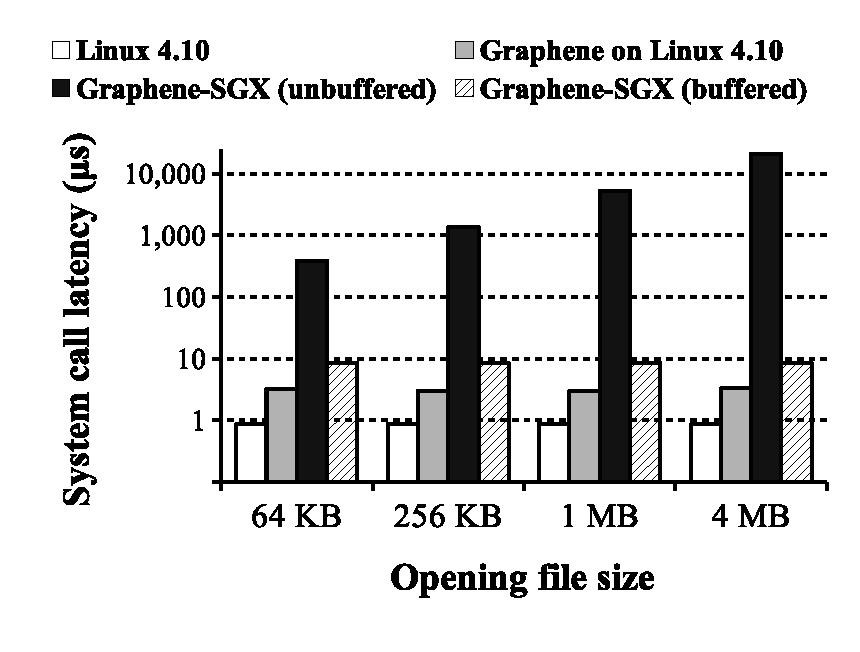
\includegraphics[width=24em]{pal/open-latency}\\
{\bf (a) Linux vs. Linux PAL}
\vspace{6pt}
\end{minipage}
\begin{minipage}{.49\linewidth}
\centering
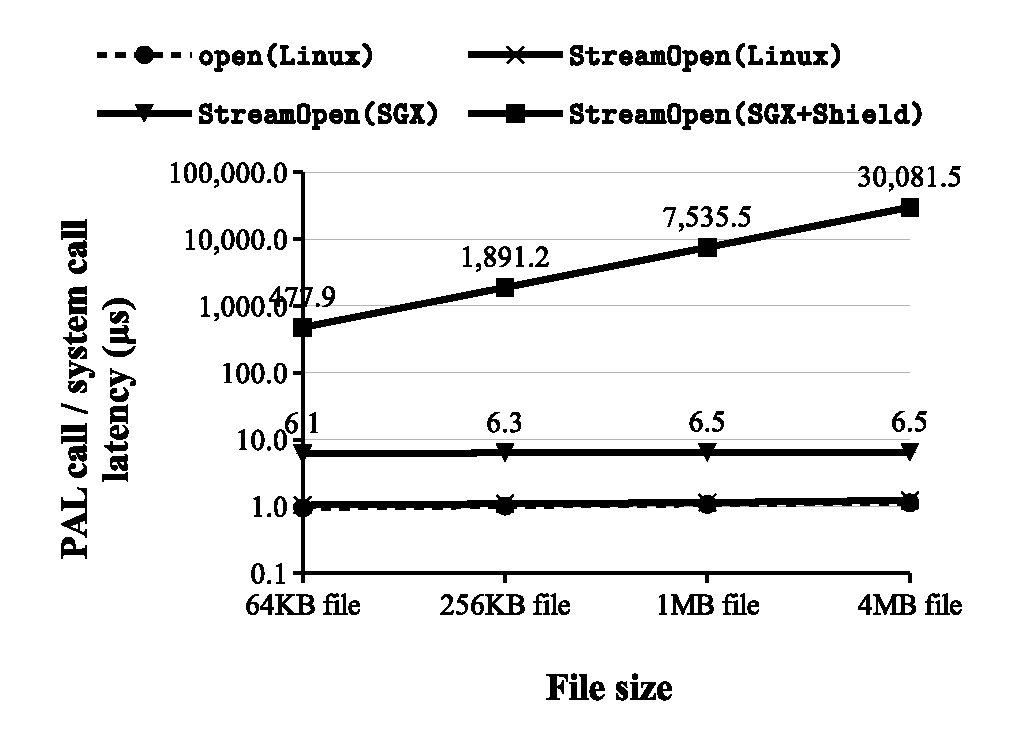
\includegraphics[width=24em]{pal/sgx-open-latency}\\
{\bf (b) Linux vs. Linux PAL vs. SGX PAL}
\vspace{6pt}
\end{minipage}
\caption{Latency of \palcall{StreamOpen} on Linux and SGX, and \syscall{open} \linuxapis{} in a native Linux process. Figure (a) shows the comparison between \syscall{open} \linuxapis{} and \palcall{StreamOpen} on a Linux PAL,
with the options of enabling the SECCOMP filter ({\bf +SC})
and reference monitor ({\bf +RM}). Figure(b) shows the comparison between  \syscall{open} \linuxapis{}, \palcall{StreamOpen} on a Linux PAL,
and \palcall{StreamOpen} inside an SGX enclave, either with or without
integrity protection ({\bf +Shield}).}
\label{fig:eval:pal:open-latency}
\end{figure*}


Figure~\ref{fig:eval:pal:open-latency} (b) shows the latency of \palcall{StreamOpen} inside of an SGX enclave, versus the latency of 
\palcall{StreamOpen} and \syscall{open} on Linux.
Without security checks to shield an enclave from the OS,
the latency of \palcall{StreamOpen} is dominated by the overhead of exiting the enclave and copying the argument out of the enclave,
for accessing the host \linuxapis{}.
The overheads of unshielded \palcall{StreamOpen} is 4.7--5.5$\times$, or \roughly{}5 \usec{}.
If a file is shielded with integrity protection,
\palcall{StreamOpen} will verify the checksum of the whole file against the manifest, and generate a Merkel Tree of file chunk hashes
for optimizing the latency of following \palcall{StreamRead} or \palcall{StreamMap}.
The overhead of enforcing the integrity check is correlated with the file size, and dominated by the time of
calculating a SHA256 hash of the file.
For a 4MB file, the latency of \palcall{StreamOpen} can be up to \roughly{}30 \msec{}.






\begin{figure*}[t!]
\centering
\footnotesize
\begin{minipage}{.49\linewidth}
\centering
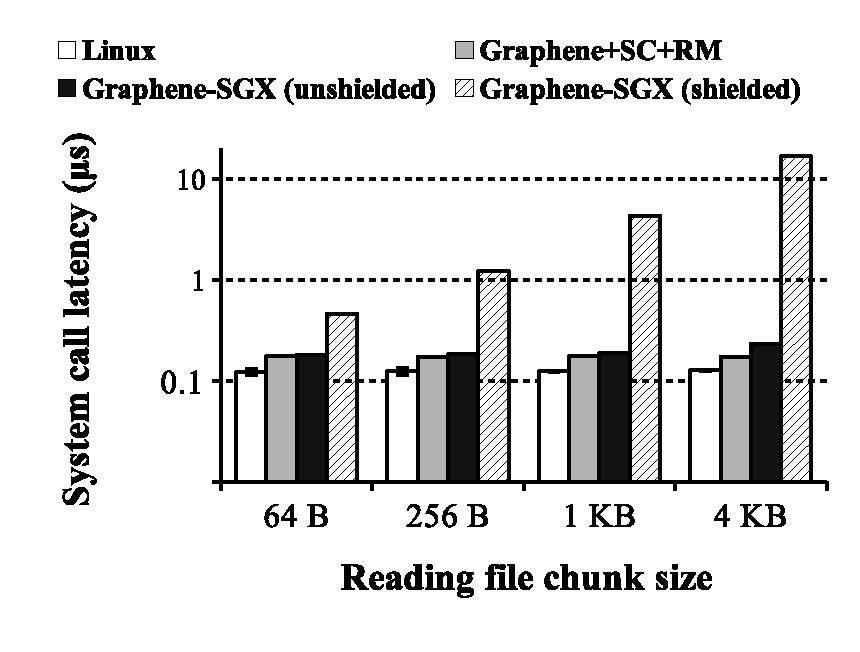
\includegraphics[width=24em]{pal/read-latency}\\
{\bf (a) Sequential read}
\vspace{6pt}
\end{minipage}
\begin{minipage}{.49\linewidth}
\centering
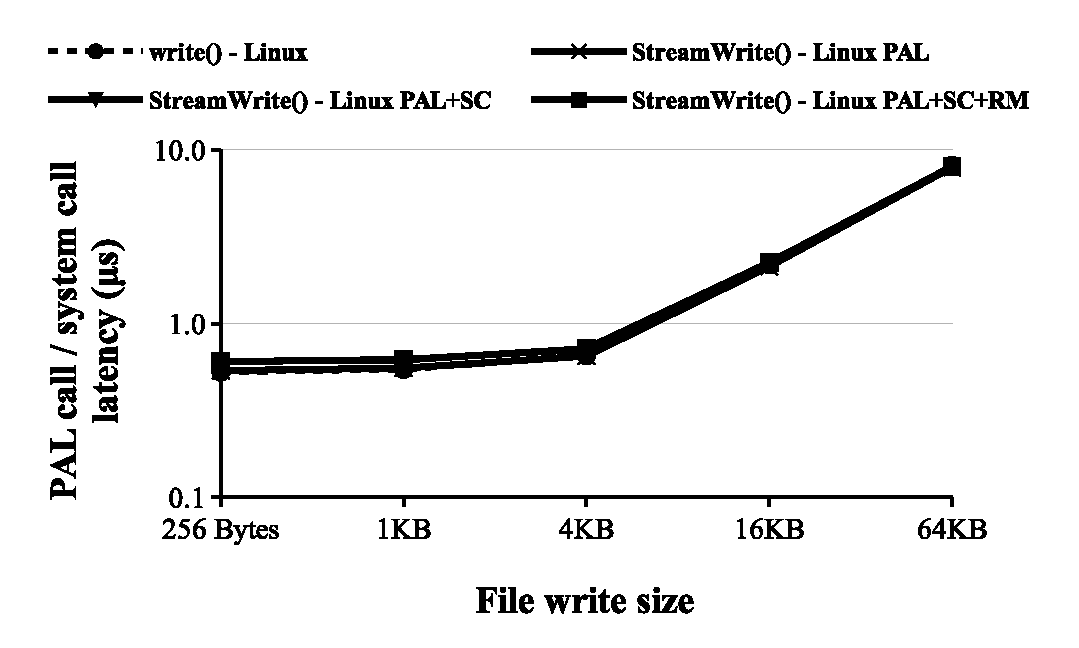
\includegraphics[width=24em]{pal/write-latency}\\
{\bf (b) Sequential write}
\vspace{6pt}
\end{minipage}
\caption{Latency of sequential \palcall{StreamRead} and \palcall{StreamWrite} on Linux, compared with the latency of \syscall{read} and \syscall{write} \linuxapis{} in a native Linux process. The comparison is between the \linuxapis{} and the \hostapis{} on a Linux PAL,
with the options of enabling the SECCOMP filter ({\bf +SC})
and reference monitor ({\bf +RM}).}
\label{fig:eval:pal:read-write-latency}
\end{figure*}

\begin{figure*}[t!]
\centering
\footnotesize
\begin{minipage}{.49\linewidth}
\centering
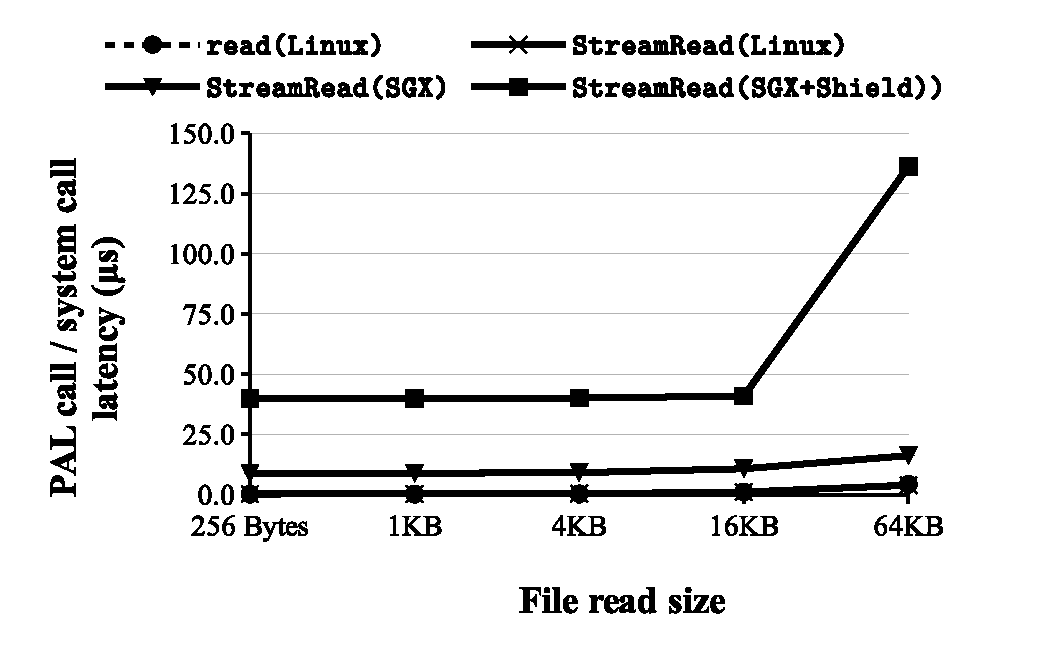
\includegraphics[width=24em]{pal/sgx-read-latency}\\
{\bf (a) Sequential read}
\vspace{6pt}
\end{minipage}
\begin{minipage}{.49\linewidth}
\centering
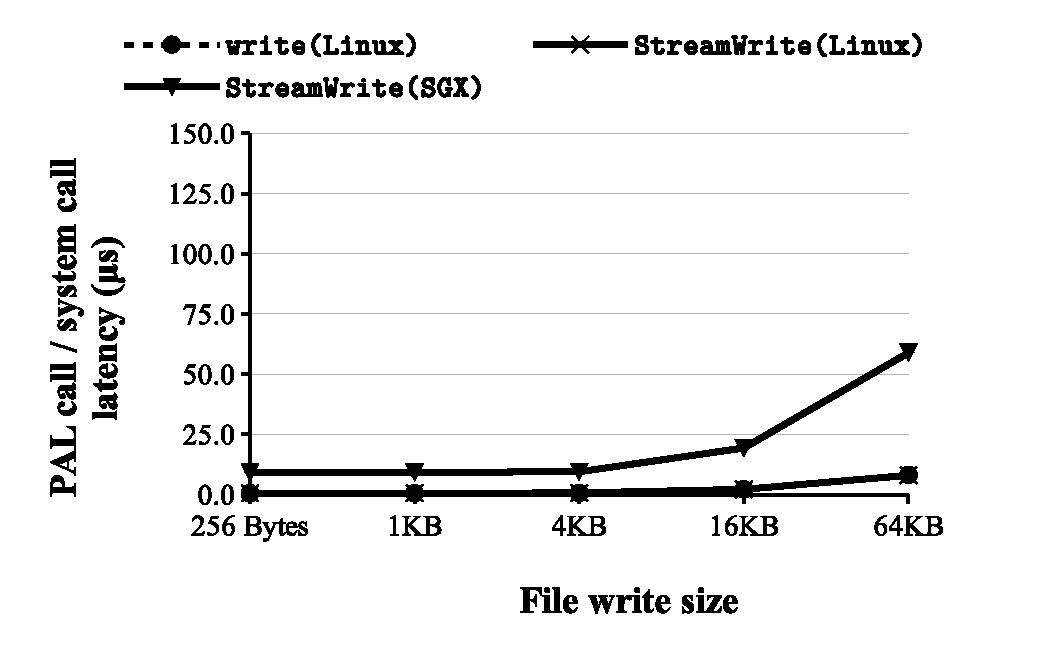
\includegraphics[width=24em]{pal/sgx-write-latency}\\
{\bf (b) Sequential write}
\vspace{6pt}
\end{minipage}
\caption{Latency of sequential \palcall{StreamRead} and \palcall{StreamWrite} inside an SGX enclave, compared with the latency of \syscall{read} and \syscall{write} \linuxapis{} in a native Linux process. The comparison is between (1) Linux \linuxapis{}; (2) \hostapis{} on a Linux PAL (without the SECCOMP filter and reference monitor); (3) \hostapis{} in an enclave, either with or without integrity protection ({\bf +Shield}).
The integrity protection for contents written by \palcall{StreamWrite}
is currently not supported.}
\label{fig:eval:pal:sgx-read-write-latency}
\end{figure*}


\paragraph{File reads and writes.}
Figure~\ref{fig:eval:pal:read-write-latency} (a) and (b) show the latency of sequential reads and writes within a 4MB file, using either Linux \linuxapis{} (\syscall{read} and \syscall{write})
or \hostapis{} (\palcall{StreamRead} and \palcall{StreamWrite}).
In general, the latency of sequential \syscall{read} and \syscall{write}
\linuxapis{} on Linux
is roughly proportional to the read and write size on the file,
especially for sizes larger than 4KB, and the latency of sequential writes can be up to twice of the latency of sequential reads by the same size. 
The Linux PAL exports \palcall{StreamRead} and \palcall{StreamWrite}
without significant overheads
for the translation to \syscall{read} or \syscall{write} \linuxapis{}.
The SECCOMP filter adds a fixed overhead around 0.06--0.09 \msec{} to the latency of \palcall{StreamRead} and \palcall{StreamWrite}.
Enabling the reference monitor has nearly no impact to the sequential read and write latency,
since the reference monitor only checks against the file access rules
when opening the file.
 

On the SGX PAL, the cryptographic operations for verifying the inputs from the untrusted OS contribute
to a major portion of the latency of \palcall{StreamRead}, similar to  \palcall{StreamOpen}. 
Figure~\ref{fig:eval:pal:sgx-read-write-latency} (a) and (b) show the latency of sequential reads and writes
inside an SGX enclave and a native Linux process,
using either \hostapis{} or \linuxapis{}.
Without integrity protection,
\palcall{StreamRead} and \palcall{StreamWrite} simply exit the enclave
to read or write the contents of a file,
and copy the contents across the enclave boundary.
The overall overhead is 8--12 \usec{} for reads and 8--50 \usec{} for writes.
The integrity protection
for \palcall{StreamRead} is based on
checking the secure hash of the file contents read from the untrusted OS,
against a Merkle tree constructed at \palcall{StreamOpen}
by hashing each 16KB block.
As a result, the latency of \palcall{StreamRead} with integrity checks is constant when the read size is smaller than 16KB, and is proportional to the number of 16KB chunks required at \palcall{StreamRead}.
The integrity protection for contents written to a host file is not yet implemented in \graphenesgx{}.





%\paragraph{Network connections.}





\paragraph{Network latency and bandwidth.}
Figure~\ref{fig:eval:pal:network-latency-bandwidth} (a) and (b) show the turnaround latency of sending single-byte messages back and forth over local TCP and UDP streams, and the bandwidth of continuously sending 64KB messages over the same TCP stream.
For the Linux PAL,
the overheads of ping-ponging over either a TCP or UDP stream primarily contribute to the translation from \hostapis{} to Linux \linuxapis{}, including \syscall{sendmsg} and \syscall{recvmsg}.
The translation costs for a TCP stream and a UDP stream inside the Linux PAL are \roughly{}18\% and \roughly{}30\%.
The overhead on the TCP bandwidth test is much lower,
at \roughly{}4\%, because the translation cost is relatively insignificant when sending larger messages. 
Besides the translation costs, the overheads of enabling the SECCOMP filter and reference monitor are both lower than 1\%, for either TCP or UDP streams.


For the SGX PAL, both the latency and bandwidth of a network stream suffer significant overheads, mostly due to enclave exits and copying network payloads inside or outside of the enclave. Note that \graphenesgx{} assumes most applications are easily configured with TLS/SSL to protect the confidentiality and integrity of network payloads; therefore, the SGX PAL currently does not implement integrated protection for network streams. The SGX PAL only checks the range of buffers
returned from the untrusted OS
to defend against pointer-based Iago attacks.
Without using cryptographic techniques to protect the contents of network streams, the overheads on the latency of ping-ponging over a TCP stream and a UDP stream are \roughly{}167\% and \roughly{}131\%, respectively, and the overhead on the TCP bandwidth test is \roughly{}79\%. 

\begin{figure*}[t!]
\centering
\footnotesize
\begin{minipage}{.56\linewidth}
\centering
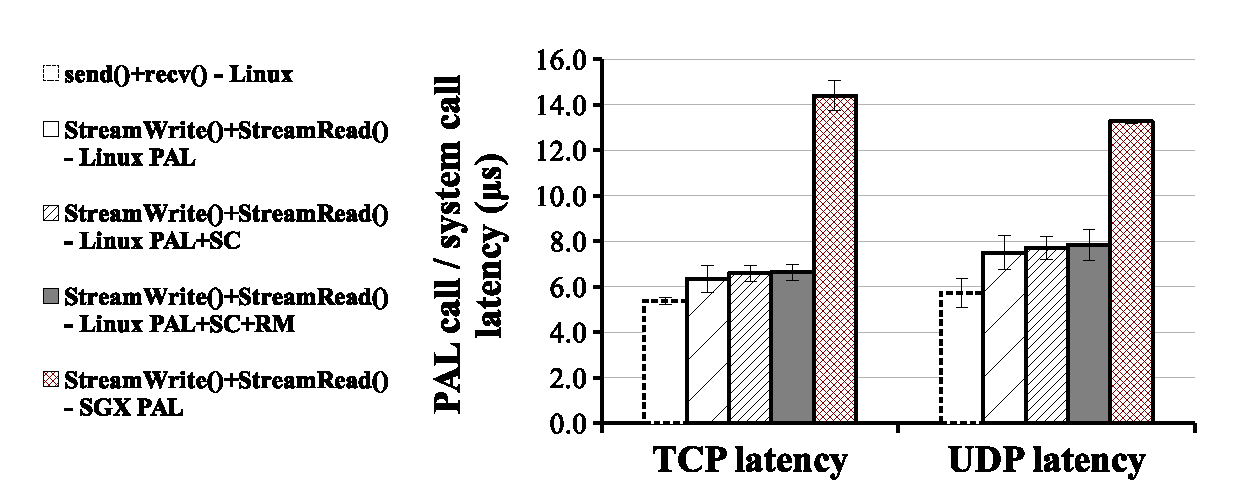
\includegraphics[width=27.2em]{pal/tcp-udp-latency}\\
{\bf (a) Latency (\usec{})}
\vspace{6pt}
\end{minipage}
\begin{minipage}{.42\linewidth}
\centering
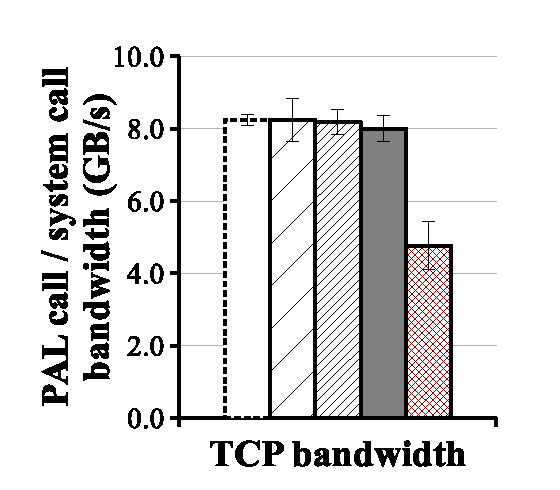
\includegraphics[width=20.4em]{pal/tcp-bandwidth}\\
{\bf (b) Bandwidth (MB/s)}
\vspace{6pt}
\end{minipage}
\caption{Latency of TCP and UDP ping-ponging, and bandwidth over a TCP stream.
The comparison is between (1) \linuxapis{} in a native Linux process; (2) \hostapis{} on a Linux PAL, with the options of enabling the SECCOMP filter ({\bf +SC}) and reference monitor ({\bf +RM}); (3) \hostapis{} in an enclave, without any shielding mechanisms.}
\label{fig:eval:pal:network-latency-bandwidth}
\end{figure*}




\paragraph{RPC latency and bandwidth.}
Figure~\ref{fig:eval:pal:pipe-latency-bandwidth} (a) and (b) show
the turnaround latency of sending single-byte messages back and forth over a local RPC stream, and the bandwidth of continuously sending 64KB messages over the same RPC stream.
For comparison, Figure~\ref{fig:eval:pal:pipe-latency-bandwidth} includes the latency and bandwidth of both normal unnamed pipes and named UNIX domain sockets.
Since the underlying implementation of RPC streams in the Linux PAL
uses UNIX domain sockets,
both the latency and bandwidth of a PRC streams
is close to a UNIX domain socket, with no significant translation cost or overheads of SECCOMP filter and reference monitor.


For the SGX PAL,
the fundamental cost of enclave exits and copying message contents,
without protecting the message contents,
is \roughly{}154\% to the latency,
or \roughly{}127\% to the bandwidth.
However, unlike network streams, \graphenesgx{} cannot assume RPC streams to be protected by inlined SSL/TLS connections
inside applications.
Since it is likely that an application may send sensitive information
over a pipe or a UNIX socket,
the underlying RPC streams must always be protected by the SGX PAL.
For each RPC streams, the SGX PAL establishes a TLS connection using a AES-GCM algorithm, which both authenticates and encrypts the message contents.
The AES-GCM algorithm in \graphenesgx{} is accelerated by the Intel AES-NI instructions, which are guaranteed to exist on a SGX-enabled CPU.
With the hardware-accelerated AES-GCM,
the overhead on the RPC latency is still up to \roughly{}335\% compared to the UNIX domain socket;
furthermore, the overhead on the RPC bandwidth
is up to \roughly{}70$\times$ (\roughly{} 176 MB/s).
Potentially switching to a more efficient cryptographic algorithm or library may improve the overheads on RPC streams,
and the experiment is left for future work.



\begin{figure*}[t!]
\centering
\footnotesize
\begin{minipage}{.49\linewidth}
\centering
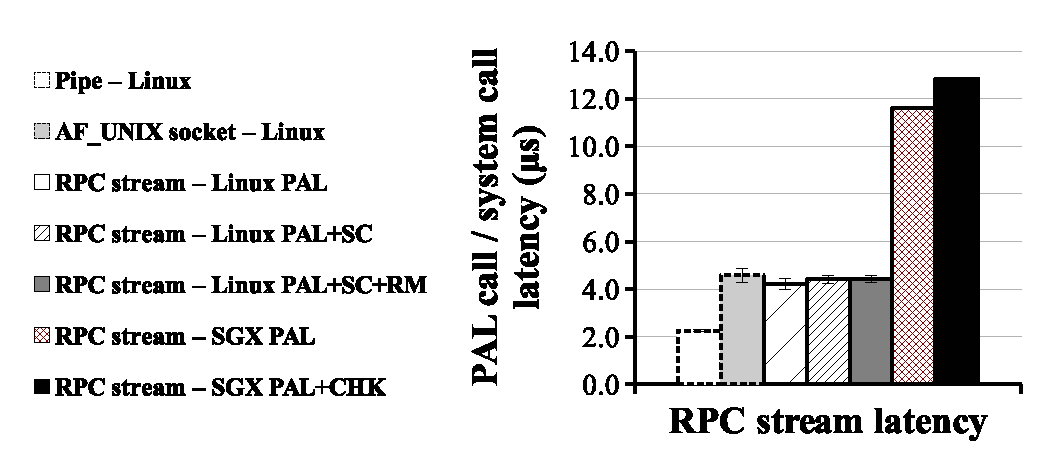
\includegraphics[width=24em]{pal/pipe-latency}\\
{\bf (a) Latency (\usec{})}
\vspace{6pt}
\end{minipage}
\begin{minipage}{.49\linewidth}
\centering
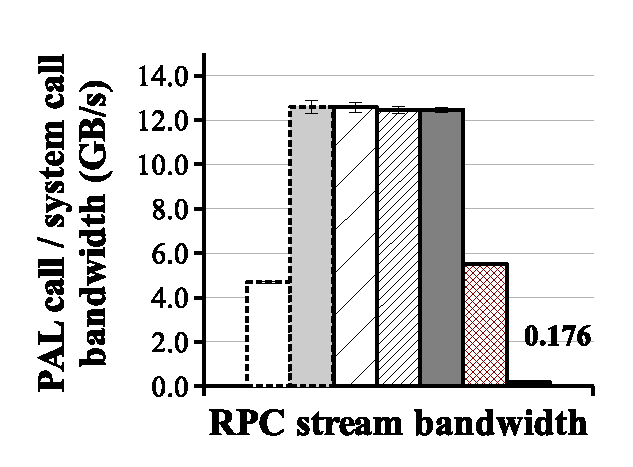
\includegraphics[width=24em]{pal/pipe-bandwidth}\\
{\bf (b) Bandwidth (MB/s)}
\vspace{6pt}
\end{minipage}
\caption{Latency of RPC ping-ponging, and bandwidth over a RPC stream.
The comparison is between (1) \linuxapis{} in a native Linux process; (2) \hostapis{} on a Linux PAL, with the options of enabling the SECCOMP filter ({\bf +SC}) and reference monitor ({\bf +RM}); (3) \hostapis{} in an enclave, without any shielding mechanisms.}
\label{fig:eval:pal:pipe-latency-bandwidth}
\end{figure*}


\paragraph{Summary.}
The efficiency of \hostapis{} for accessing files or I/O streams
inevitably suffers some overheads,
due to the nature of these abstractions to be sharable
among applications.
Each of these \hostapis{} externalizes certain guest OS states
%such as buffered file contents or network payloads,
to the host OS,
using the existing host system interfaces.
Most of the experiment results
show that the translation cost between the \hostapis{} and the host system interfaces can be reduced
by mitigating the needs of reconstructing the \hostapi{} arguments
and copying stream buffers.
Only a few exceptions, such as the translation of URIs to network addresses,
or copying the arguments or buffers in or out of an enclave,
cause more significant overheads to the overhead of these \linuxapis{}.




Security checks, either in the host kernel or inside an enclave,
often contribute to
non-trivial overheads on the \hostapis{} for accessing I/O streams.
The cost of security checks
varies between different threat models.
For the Linux PAL, the cost includes the overhead of enabling a SECCOMP filter, and the cost of checking file paths and network addresses
inside of an reference monitor.
With the JIT (Just-in-time) optimization,
the overheads of SECCOMP filter is generally less than 10\%.
The overheads of security monitors can range from 0--21\%, but only impact \hostapis{} which accept an URI as argument (e.g., \palcall{StreamOpen} and \palcall{StreamAttrQuery}).

 
The SGX PAL further adopts several cryptographic techniques
for protecting the confidentiality and integrity of I/O streams, which impose significant overheads.
Verifying the file contents, either at first open of the file or consequential file reads,
causes 500--24,000$\times$ overheads on \palcall{StreamOpen}
or 25--150$\times$ overheads on \palcall{StreamRead}.
Authenticating and encrypting a RPC stream, using a TLS connection with hardware-accelerated AES-GCM algorithm,
causes \roughly{}335\% overhead beyond the latency of underlying UNIX domain sockets,
or \roughly{}70 $\times$ overhead on bandwidth when sending large messages.






\subsection{Page management}


Figure~\ref{fig:eval:pal:mmap-latency} (a)
shows the combined latency of \palcall{VirtMemAlloc} and  \palcall{VirtMemFree}, on both Linux and SGX PALs,
and the latency of \syscall{mmap} and \syscall{munmap} in a native Linux process.
The latency of both \syscall{mmap}+\syscall{munmap} and \syscall{VirtMemAlloc}+\syscall{VirtMemFree} on Linux is partially correlated with the size of memory mapped inside a process or \picoproc{}.
Due to the similarity between the \hostapis{} and the \linuxapis{},
the translation cost is almost marginal
to the latency of allocating and deallocating the memory mappings.
Enabling the SECCOMP filter adds an additional
15--25\% overhead to the latency of \syscall{VirtMemAlloc}+\syscall{VirtMemFree}, which is common for all \linuxapis{} used by the Linux PAL.
However, if the latency includes zeroing the allocated memory mappings,
which triggers the population of physical pages
inside the host kernel,
the overhead is much more significant and proportional to the mapping size.
As a result, allocating, accessing, and deallocating a 64MB memory mapping will take up to \roughly{}3.5\msec{}.


For the SGX PAL, the latency of allocating and deallocating memory mapping
is much lower then the Linux PAL, because the SGX PAL does not dynamically allocate the enclave memory region.
Due the limitation of current SGX hardware,
the SGX PAL must implement memory mappings internally,
with all the enclave page populated and signed by the CPU before the enclave starts execution.
Based on this design, the latency of \syscall{VirtMemAlloc}+\syscall{VirtMemFree} on the SGX PAL
is 8--11\% of the latency on the Linux PAL,
since these two \hostapis{} only update the memory mapping records inside the enclave.
However, if the enclave memory is accessed immediately after allocation, as shown in Figure~\ref{fig:eval:pal:mmap-latency} (b),
the overhead can be up to 3--9.5$\times$, and is proportional to the size of memory mappings.

\begin{figure*}[t!]
\centering
\footnotesize
\begin{minipage}{.49\linewidth}
\centering
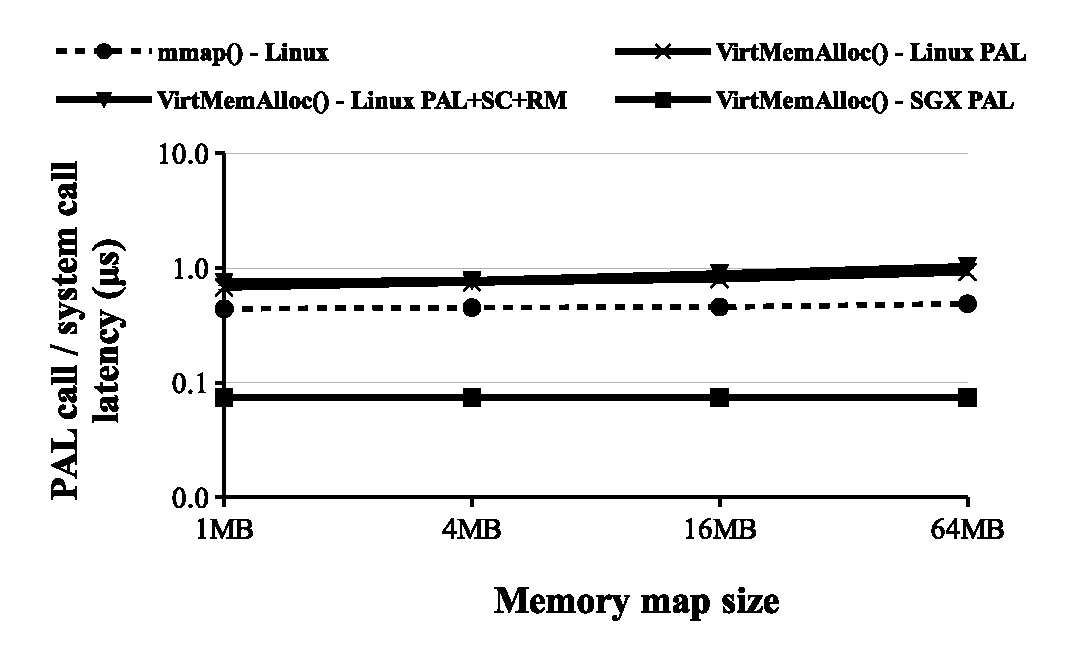
\includegraphics[width=24em]{pal/mmap-latency}\\
{\bf (a) allocation + deallocation}
\vspace{6pt}
\end{minipage}
\begin{minipage}{.49\linewidth}
\centering
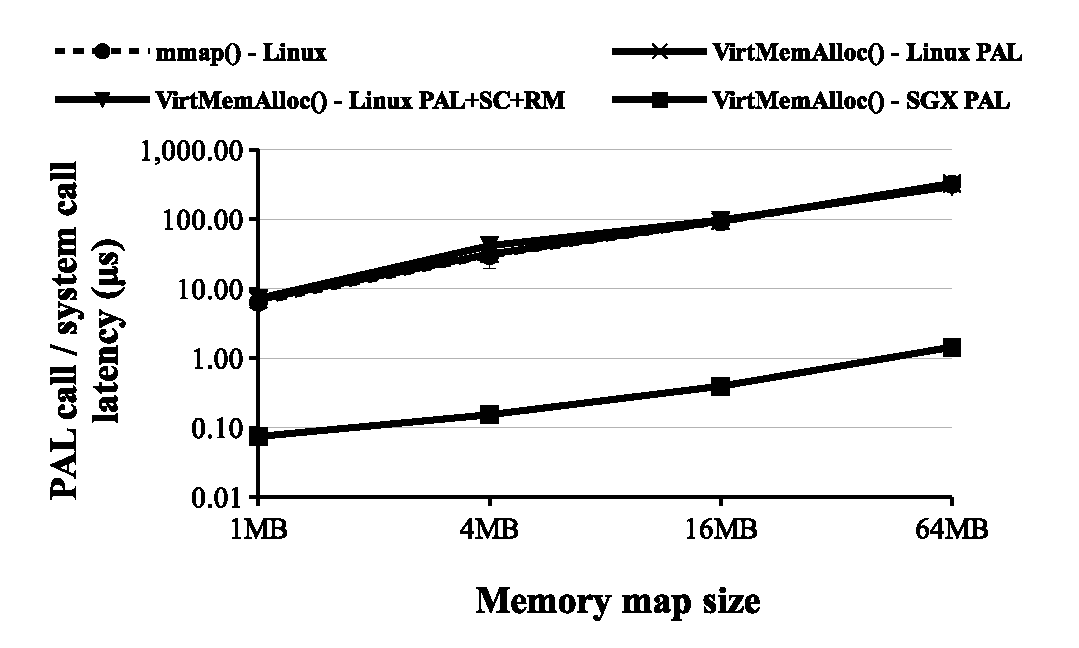
\includegraphics[width=24em]{pal/mmap-access-latency}\\
{\bf (b) allocation + memory access + deallocation}
\vspace{6pt}
\end{minipage}
\caption{Latency of allocating and deallocating memory mappings, using either \syscall{mmap} and \syscall{munmap} on Linux, or \palcall{VirtMemAlloc} and \palcall{VritMemFree} on the Linux and SGX PALs.
(a) shows the combined latency of allocation and deallocation, whereas (b) includes the latency of zeroing memory pages.
%which triggers the host kernel to populate the physical pages. 
The comparison is between (1) \linuxapis{} in a native Linux process; (2) \hostapis{} on a Linux PAL, with the options of enabling the SECCOMP filter ({\bf +SC}) and reference monitor ({\bf +RM}); (3) \hostapis{} in an enclave. No shielding mechanism is needed.}
\label{fig:eval:pal:mmap-latency}
\end{figure*}

To sum up, the evaluation results on \syscall{VirtMemAlloc} and \syscall{VirtMemFree}
show that the Linux PAL share the same latency
with a native Linux process
for creating virtual memory mappings, paging and memory access.
On the other hand, despite that the SGX PAL manages all the enclave pages
inside the enclave,
the SGX PAL suffers a larger overhead for paging and bringing memory into the last-level cache.



\subsection{Scheduling}




\begin{figure*}[t!]
\centering
\footnotesize
\begin{minipage}{.44\linewidth}
\centering
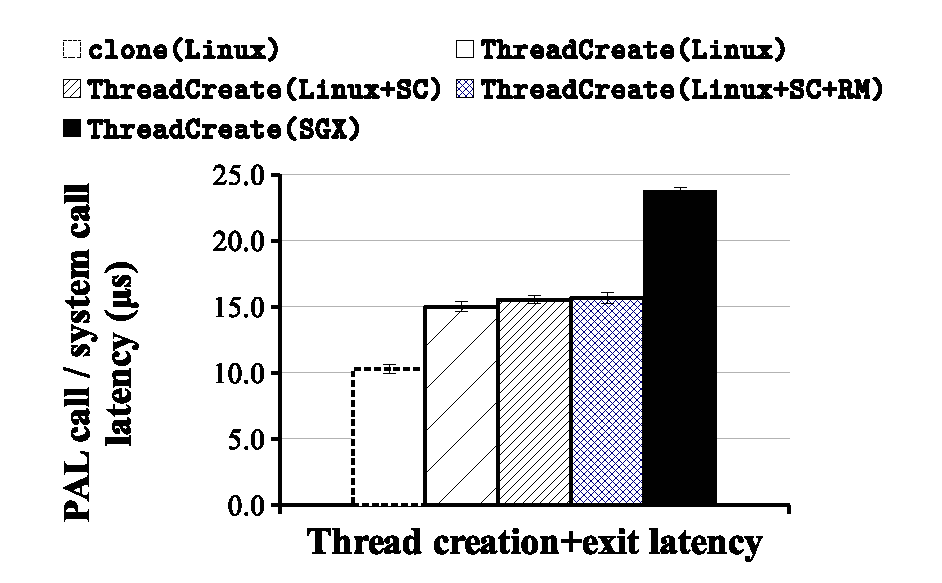
\includegraphics[width=24em]{pal/thread-latency}\\
{\bf (a) thread creation}
\vspace{6pt}
\end{minipage}
\begin{minipage}{.54\linewidth}
\centering
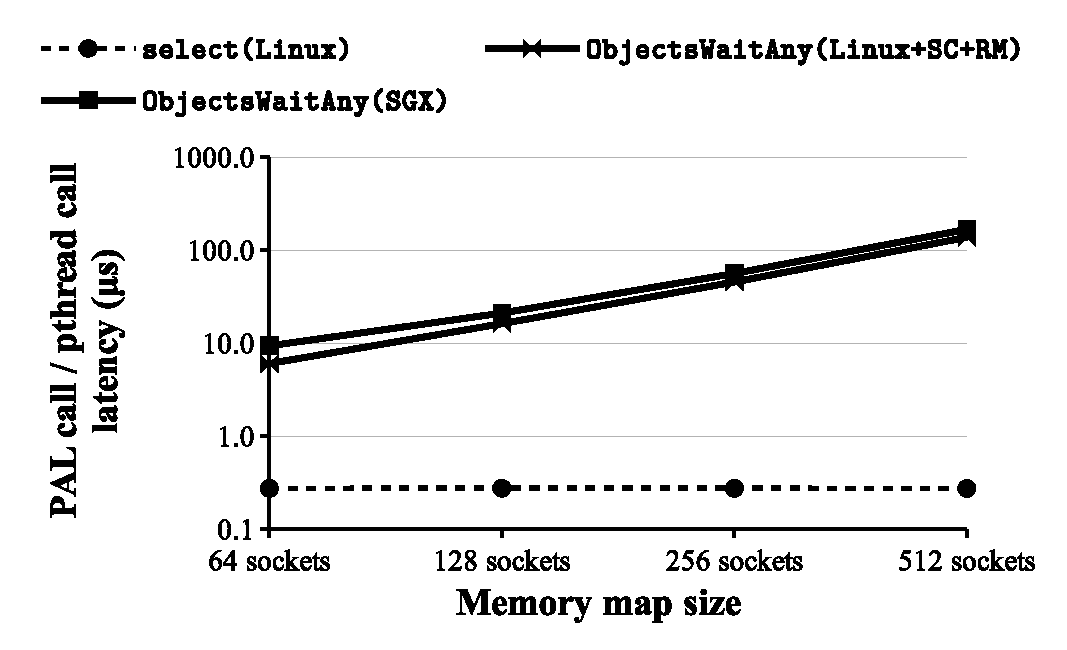
\includegraphics[width=25em]{pal/tcp-select-latency}\\
{\bf (b) polling TCP sockets}
\vspace{6pt}
\end{minipage}
\caption{Latency of allocating and deallocating memory mappings, using either \syscall{mmap} and \syscall{munmap} on Linux, or \palcall{VirtMemAlloc} and \palcall{VritMemFree} on the Linux and SGX PALs.
(a) shows the combined latency of allocation and deallocation, whereas (b) includes the latency of zeroing memory pages.
%which triggers the host kernel to populate the physical pages. 
The comparison is between (1) \linuxapis{} in a native Linux process; (2) \hostapis{} on a Linux PAL, with the options of enabling the SECCOMP filter ({\bf +SC}) and reference monitor ({\bf +RM}); (3) \hostapis{} in an enclave. No shielding mechanism is needed.}
\label{fig:eval:pal:thread-select-latency}
\end{figure*}






\begin{figure*}[t!]
\centering
\footnotesize
\begin{minipage}{.49\linewidth}
\centering
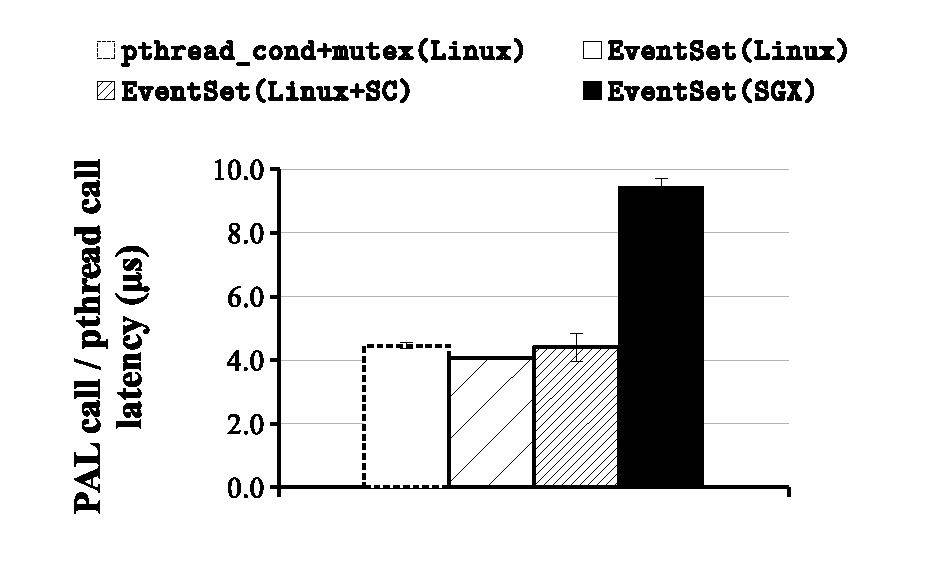
\includegraphics[width=24em]{pal/event-latency}\\
{\bf (a) allocation + deallocation}
\vspace{6pt}
\end{minipage}
\begin{minipage}{.49\linewidth}
\centering
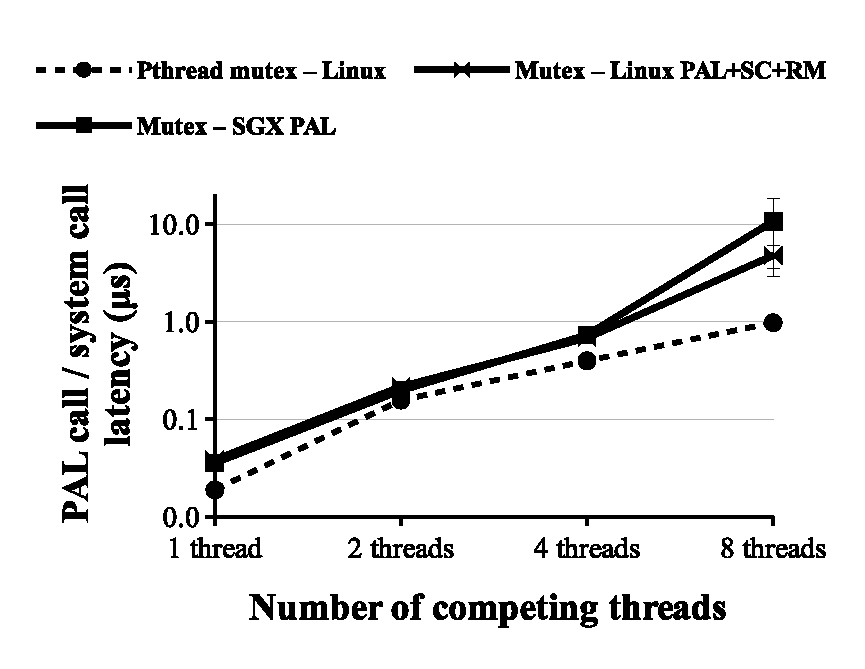
\includegraphics[width=24em]{pal/mutex-latency}\\
{\bf (b) allocation + memory access + deallocation}
\vspace{6pt}
\end{minipage}
\caption{Latency of allocating and deallocating memory mappings, using either \syscall{mmap} and \syscall{munmap} on Linux, or \palcall{VirtMemAlloc} and \palcall{VritMemFree} on the Linux and SGX PALs.
(a) shows the combined latency of allocation and deallocation, whereas (b) includes the latency of zeroing memory pages.
%which triggers the host kernel to populate the physical pages. 
The comparison is between (1) \linuxapis{} in a native Linux process; (2) \hostapis{} on a Linux PAL, with the options of enabling the SECCOMP filter ({\bf +SC}) and reference monitor ({\bf +RM}); (3) \hostapis{} in an enclave. No shielding mechanism is needed.}
\label{fig:eval:pal:mmap-latency}
\end{figure*}




\subsection{Multi-process abstractions}













\subsection{Miscellaneous}

